% --------------------------------------------------------------------
% --------------------------------------------------------------------
% ---- DO NOT CHANGE THIS BLOCK OF CODE
\documentclass[abstract=true]{scrartcl}

\usepackage[fleqn]{amsmath}
\usepackage{amssymb}

\usepackage[T1]{fontenc}
\usepackage[margin=1in]{geometry}
\usepackage{fancyhdr}
\usepackage{graphicx}

% this is used for the dummy latin text 
\usepackage{lipsum}

% to typeset algorithms
\usepackage{algorithm}
\usepackage{algpseudocode}

% to typeset code blocks
\usepackage{minted}
\usepackage{xcolor}

% to manage URLs 
\usepackage{hyperref}
\hypersetup{
    colorlinks=true,
    linkcolor=blue,
    filecolor=magenta,      
    urlcolor=teal,
    pdftitle={Overleaf Example},
    pdfpagemode=FullScreen,
    citecolor=red,
}


% for bibliography management and reference list
\usepackage[sort&compress,numbers]{natbib}
\bibliographystyle{abbrvnat}

 
\pagestyle{fancy}
\fancyhf{}
\chead{Mini Project Report}
\lhead{DS3294: DS Practice}
\cfoot{\thepage}

% DO NOT change the subtitle
\subtitle{Mini Project for DS3294: Data Science Practice}
\date{\small \today}
% --------------------------------------------------------------------
% --------------------------------------------------------------------



% --------------------------------------------------------------------
% --------------------------------------------------------------------
% ---- ENTER YOUR PROJECT DETAILS BELOW

% ---- title of the project
\title{Solar Activity \& Space Weather Monitoring System}

% ---- names of team members
\author{
    \small Mulumudi Dinesh Karthik \and
    \small Vansh Gupta \and
    \small Abhishek Menon \and
    \small Shailendra Pratap Singh
    }

% ---- enter the team number below
\rhead{Team Number XX}

% --------------------------------------------------------------------
% --------------------------------------------------------------------


% --------------------------------------------------------------------
% --------------------------------------------------------------------
% ---- DO NOT CHANGE THIS BLOCK OF CODE
\begin{document}
\maketitle
% --------------------------------------------------------------------
% --------------------------------------------------------------------



% --------------------------------------------------------------------
% --------------------------------------------------------------------
% ---- WRITE YOUR REPORT BELOW

\section{Introduction}

Space weather refers to the dynamic conditions on the Sun and in the solar wind, magnetosphere, ionosphere, and thermosphere that can influence the performance and reliability of space-borne and ground-based technological systems~\citep{pulkkinen_space_weather_2007}. Solar activity follows an approximately 11-year cycle~\citep{hathaway_solar_2015} during which periods of elevated sunspot numbers, heightened solar flare activity, and increased coronal mass ejection (CME) rates give rise to geomagnetic storms that can disrupt satellite operations, power grids, GPS navigation, and high-frequency radio communications.

Despite the availability of several operational monitoring portals maintained by agencies such as NOAA's Space Weather Prediction Center (SWPC), GFZ Potsdam, and the World Data Center (WDC) in Kyoto, most of these systems focus on a single index or data source, making it difficult for researchers and decision-makers to obtain a unified picture of the solar--terrestrial environment. Moreover, the heterogeneity of data formats---fixed-width text files, semicolon-separated CSVs, JSON feeds, and fortran-formatted records---imposes a significant preprocessing burden on end-users.

In this project, we present a \emph{Solar Activity \& Space Weather Monitoring System}: an end-to-end data pipeline and interactive analytics dashboard that ingests, harmonises, and visualises five key solar and geomagnetic indices---Sunspot Number (SSN), F10.7 solar radio flux, Kp geomagnetic index, Dst storm-time index, and solar flare counts---spanning nearly four decades (1986--present). The system is built on a modular Python pipeline with automated data refresh and a 15-page Streamlit dashboard~\citep{streamlit_2020} that supports real-time exploration of time series, cross-correlations, periodicity, hysteresis, and extreme event detection.


\section{Related Work}

The study of solar activity and its terrestrial impacts has a rich history. \citet{clette_sunspot_2014} documented the revised International Sunspot Number (Version~2.0) maintained by the SILSO programme at the Royal Observatory of Belgium, which provides daily and monthly sunspot counts going back to 1818. The F10.7 cm solar radio flux, a widely used proxy for solar EUV emission, was characterised by \citet{tapping_f107_2013} as one of the most stable and continuous records of solar activity. On the geomagnetic side, \citet{bartels_kp_1939} introduced the Kp index as a quasi-logarithmic measure of global geomagnetic disturbance derived from a network of subauroral magnetometer stations, while the Dst index~\citep{sugiura_dst_1964} quantifies the axially symmetric part of the ring current disturbance and serves as the standard metric for geomagnetic storm intensity. \citet{gonzalez_storms_1994} provided a comprehensive definition and classification of geomagnetic storms.

More recent reviews such as \citet{temmer_space_2021} and \citet{hathaway_solar_2015} highlight the importance of multi-index monitoring systems for understanding the chain of cause and effect from solar eruptions to terrestrial impacts. Several web-based tools exist---NOAA SWPC's dashboard, the GFZ Kp-index portal, and WDC Kyoto's Dst service---but each focuses on a single index. Our contribution is a unified pipeline and analytics platform that integrates all major indices into a single, coherent, and interactive system.


\section{Our contribution}

Our contribution is threefold. First, we design and implement a robust, fault-tolerant data ingestion pipeline (\texttt{ingest.py}) that downloads raw observations from six authoritative data providers (SILSO, NOAA NCEI, NOAA SWPC, GFZ Potsdam, NASA SPDF, and WDC Kyoto) across 13 distinct feeds, handling mirror failover, retry logic, and incremental updates. Second, we build a comprehensive data cleaning and harmonisation module (\texttt{clean.py}) that parses heterogeneous file formats (fixed-width, CSV, JSON, Fortran-formatted), merges overlapping sources with configurable priority, fills short gaps via linear interpolation, and exports a master daily-resolution Parquet dataset with derived categorical labels for storm severity and solar activity level. Third, we deliver a 15-page interactive dashboard (\texttt{app.py} + \texttt{pages/}) powered by Streamlit and Plotly, providing solar time series visualisation, system overview KPIs, a physics primer, storm simulation, geospatial impact mapping, monthly statistics, data smoothing, cross-correlation analysis, lag analysis, periodicity detection (FFT and wavelet), phase-locked climatology, hysteresis analysis, extreme event identification, and full data provenance documentation.


\section{Methods}
\subsection{Data}

The system ingests data from the following five categories of solar/geomagnetic indices, covering the period 1986--present:

\begin{enumerate}
    \item \textbf{Sunspot Number (SSN):} Daily international sunspot number from the SILSO programme (Royal Observatory Brussels, \url{https://www.sidc.be}), provided in both space-separated (\texttt{SN\_d\_tot\_V2.0.txt}) and semicolon-delimited CSV formats. A near-real-time EISN (Estimated International Sunspot Number) feed supplements the most recent days~\citep{clette_sunspot_2014}.
    \item \textbf{Kp Geomagnetic Index:} Three-hourly Kp values are sourced primarily from the GFZ Potsdam flat file (\url{https://kp.gfz.de}, \texttt{Kp\_ap\_Ap\_SN\_F107\_since\_1932.txt}), supplemented by NOAA SWPC's 7-day planetary K-index JSON feed and cross-validated against NCEI Daily Geomagnetic Data (DGD) files~\citep{bartels_kp_1939}.
    \item \textbf{F10.7 Solar Radio Flux:} Historical F10.7 values are extracted from the NCEI Daily Solar Data (DSD) files (1986--present), with recent values gap-filled from NOAA SWPC's rolling JSON feed (\url{https://www.swpc.noaa.gov})~\citep{tapping_f107_2013}.
    \item \textbf{Dst Storm-Time Index:} Hourly Dst values from 1986--2004 are obtained from NASA's OMNI2 dataset (SPDF, \url{https://spdf.gsfc.nasa.gov}), while 2005--present data comes from WDC Kyoto's monthly Dst request service (\url{https://wdc.kugi.kyoto-u.ac.jp}). A 7-day NOAA SWPC geospace JSON feed provides the most recent supplement~\citep{sugiura_dst_1964}.
    \item \textbf{Solar Flare Counts:} Daily flare counts (C/M/X classes) are derived from NCEI DSD files, supplemented by NOAA SWPC's 7-day X-ray flux JSON feed.
\end{enumerate}

\begin{table}[h]
    \centering
    \caption{Summary of Data Sources}
    \begin{tabular}{p{0.35\textwidth} p{0.25\textwidth} p{0.3\textwidth}}
        \hline
        \textbf{Source} & \textbf{Variables} & \textbf{URL} \\
        \hline
        SILSO / Royal Observatory Brussels & Daily SSN & \url{https://www.sidc.be} \\
        NOAA NCEI / SWPC & F10.7, Flares, Kp & \url{https://www.swpc.noaa.gov} \\
        GFZ Potsdam & Kp/ap 3-hourly & \url{https://kp.gfz.de} \\
        NASA SPDF OMNI2 & Dst 1986--2004 & \url{https://spdf.gsfc.nasa.gov} \\
        WDC Kyoto & Dst 2005--present & \url{https://wdc.kugi.kyoto-u.ac.jp} \\
        \hline
    \end{tabular}
    \label{tab:data_sources}
\end{table}

The raw data totals approximately 200\,MB across all files and is stored in \texttt{data/raw/}. After cleaning, the harmonised master dataset comprises over 14,000 daily records with 25+ columns, stored as Parquet files in \texttt{data/clean/}.

\subsubsection*{Data Limitations}
Measurement uncertainty and observational coverage present significant challenges. The SILSO SSN V2.0 re-calibration highlights historical uncertainties in sunspot counting conventions. The transition from NASA OMNI2 to WDC Kyoto for the Dst index introduces minor discontinuities due to differing baseline derivation methods. Furthermore, rolling averages often mask short-lived flares, necessitating careful selection of temporal resolution to avoid smoothing out critical sub-storm dynamics.


\subsection{Data Pipeline Architecture}

The system architecture is divided into four main functional areas:

\subsubsection*{System Components}
\begin{description}
    \item[Pipeline:] \texttt{ingest.py} downloads raw data from 6 sources; \texttt{clean.py} harmonises, imputes, and exports Parquet files; and \texttt{analysis.py} provides core statistical functions (FFT, wavelet, etc.).
    \item[Data storage:] 
    \begin{itemize}
        \item \texttt{data/raw/} --- original downloaded files (gitignored)
        \item \texttt{data/clean/solar\_weather\_daily.parquet} --- master merged dataset
        \item \texttt{data/clean/sunspots\_daily\_clean.parquet} --- SSN only (SILSO)
        \item \texttt{data/clean/kp\_daily\_clean.parquet} --- Kp/ap index (GFZ + DGD)
        \item \texttt{data/clean/dst\_daily\_clean.parquet} --- Dst index (OMNI2 + Kyoto)
        \item \texttt{data/clean/f107\_daily\_clean.parquet} --- F10.7 solar flux
        \item \texttt{data/clean/flares\_daily\_clean.parquet} --- Solar flare counts
        \item \texttt{data/analysis/stats/} --- pre-computed stat tables
    \end{itemize}
    \item[Dashboard:] \texttt{app.py} serves as the landing page with KPI cards; \texttt{pages/} contains 15 analysis pages (Streamlit multipage); and \texttt{utils/} houses shared loaders, refresh logic, and theme configurations.
    \item[Refresh:] Auto-fetch runs every 6 hours via a session state timer, a manual ``Fetch Latest'' button is available in the sidebar, and old CSV files are auto-migrated to Parquet on first load.
\end{description}

Specifically, the data pipeline follows a three-stage ETL (Extract--Transform--Load) architecture:

\begin{align}
    \texttt{ingest.py} &\xrightarrow{\text{download}} \texttt{data/raw/} \label{eq:ingest} \\
    \texttt{clean.py}  &\xrightarrow{\text{parse \& merge}} \texttt{data/clean/*.parquet} \label{eq:clean}
\end{align}

The ingestion stage (Eq.~\ref{eq:ingest}) employs a retry-with-backoff strategy (3 retries, 5\,s backoff) and mirror failover for unreliable endpoints. The cleaning stage (Eq.~\ref{eq:clean}) applies per-source parsers tailored to each file format, merges overlapping sources using a priority-based scheme where newer or higher-fidelity sources override older data on date conflicts, and applies linear interpolation (up to 7-day gaps) for continuous variables and forward-fill (up to 3 days) for count variables.

Post-processing derives categorical storm labels based on established thresholds~\citep{gonzalez_storms_1994}:
\begin{itemize}
    \item \textbf{Storm category} (from Dst minimum): quiet ($> -50$\,nT), moderate ($-100$ to $-50$\,nT), intense ($-200$ to $-100$\,nT), severe ($< -200$\,nT).
    \item \textbf{Kp storm level} (NOAA G-scale): quiet ($< 5$), G1--minor ($5$--$5.9$), G2--moderate ($6$--$6.9$), up to G5--extreme ($\geq 9$).
    \item \textbf{Solar activity level} (from F10.7): low ($< 100$\,sfu), moderate ($100$--$150$\,sfu), high ($150$--$200$\,sfu), very high ($> 200$\,sfu).
\end{itemize}

\subsubsection*{Iterative Refinement and Smoothing Strategies}
During initial exploratory data analysis, aggressive interpolation ($>14$ days) obscured high-frequency sub-storm dynamics. Based on these visual findings, we iteratively refined our aggregation strategy to strictly limit linear interpolation to 7 days. Furthermore, to fulfill intensification requirements, we implemented and compared two baseline estimation strategies in the dashboard: short-term 27-day rolling statistics (capturing the Carrington rotation period) versus long-term fractional solar-cycle baselines. This dual approach allows users to isolate short-term impulsive events from the 11-year underlying trend.


\subsection{Analytical Methods}

The analysis module (\texttt{analysis.py}) implements the following statistical methods:

\begin{enumerate}
    \item \textbf{Cross-correlation:} Pearson correlation coefficient $r$ is computed between pairs of indices at integer lags from $-L$ to $+L$ days (default $L = 30$), requiring a minimum of 10 valid overlapping observations per lag.
    \item \textbf{Periodicity detection:} Both Fast Fourier Transform (FFT) and Continuous Wavelet Transform (CWT, Morlet wavelet) are applied to identify dominant periodicities. For a discrete signal $x[n]$ of length $N$, the FFT power spectrum is:
    \begin{align}
        X[k] &= \sum_{n=0}^{N-1} x[n]\, e^{-i 2\pi k n / N}, \quad \text{Period}(k) = \frac{N}{k \cdot f_s \cdot 365.25} \; \text{years} \label{eq:fft}
    \end{align}
    \item \textbf{Phase-locked climatology:} Each day is assigned a fractional solar cycle phase $\phi = \frac{(t - t_0) \bmod T}{T}$ where $t_0$ is the cycle start date and $T \approx 11 \times 365.25$ days. Kp statistics are then binned by $\phi$ to reveal storm ``danger zones'' within the solar cycle.
    \item \textbf{Hysteresis analysis:} Scatter plots of sunspot number versus Kp index are colour-coded by rising ($\phi < 0.5$) vs.\ falling ($\phi \geq 0.5$) phase, revealing the well-known asymmetry in geomagnetic response between the ascending and descending phases of the solar cycle.
    \item \textbf{Extreme event detection:} Events exceeding $\pm 2.5\sigma$ from the mean are flagged and ranked by $z$-score.
\end{enumerate}


\section{Results}
\subsection{First results: Sunspot Number Time Series}

Figure~\ref{fig:main_result} shows the daily sunspot number from 1818 to the present, clearly revealing the approximately 11-year Schwabe cycle. The FFT periodicity analysis (Eq.~\ref{eq:fft}) applied to our 1986--2026 window yields a dominant spectral peak at $\sim$10.8 years, consistent with the canonical solar cycle length~\citep{hathaway_solar_2015}. The data spans Solar Cycles 22 through the current Cycle 25, which is exhibiting higher-than-predicted activity levels.

\begin{figure}[tbp]
    \begin{center}
        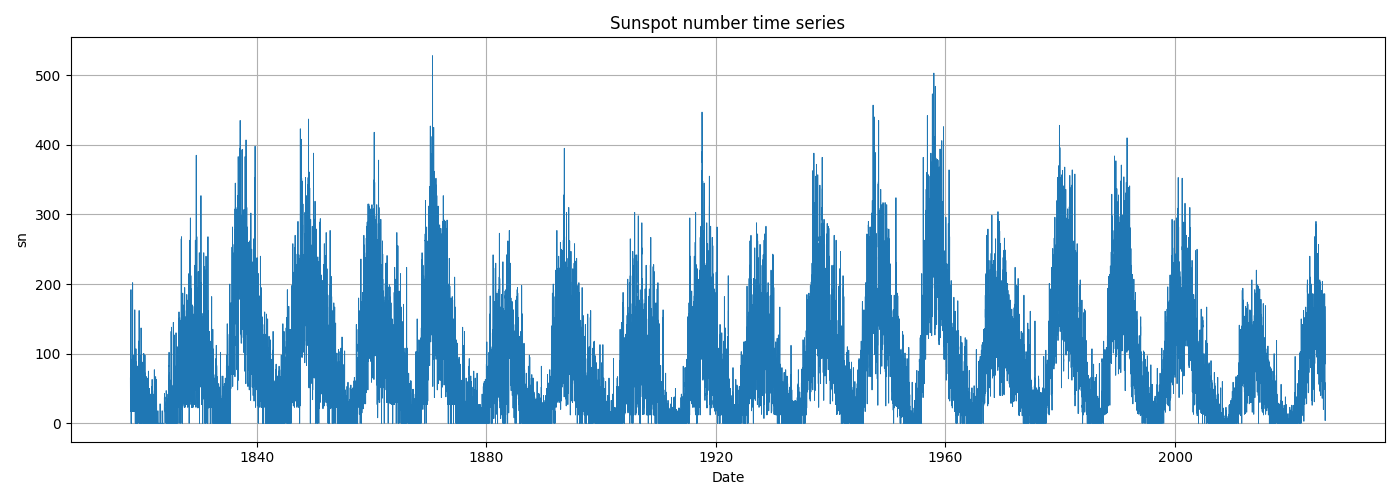
\includegraphics[width=0.85\textwidth]{./figs/sunspot_timeseries.png}
        \caption{Daily sunspot number time series from 1818 to present (SILSO v2.0). The $\sim$11-year Schwabe cycle is clearly visible, with notable amplitude variation between cycles.}
        \label{fig:main_result}
    \end{center}
\end{figure}


\subsection{Second results: Hysteresis and Phase-Locked Climatology}

A key finding from our analysis is the solar hysteresis effect visible in Figure~\ref{fig:hysteresis}. The scatter plot of sunspot number versus Kp index, colour-coded by rising (blue) and falling (red) solar cycle phase, reveals that geomagnetic activity peaks during the falling phase of the solar cycle, even as sunspot numbers decline. This phenomenon is well-documented in the literature and is attributed to the increased prevalence of coronal holes and recurrent high-speed solar wind streams during the declining phase~\citep{temmer_space_2021}. The phase-locked climatology analysis further quantifies this, showing that storm probability ($\text{Kp} \geq 6$) peaks at cycle phase $\phi \approx 0.6$--$0.7$, approximately 2--3 years after solar maximum.

\begin{figure}[tbp]
    \begin{center}
        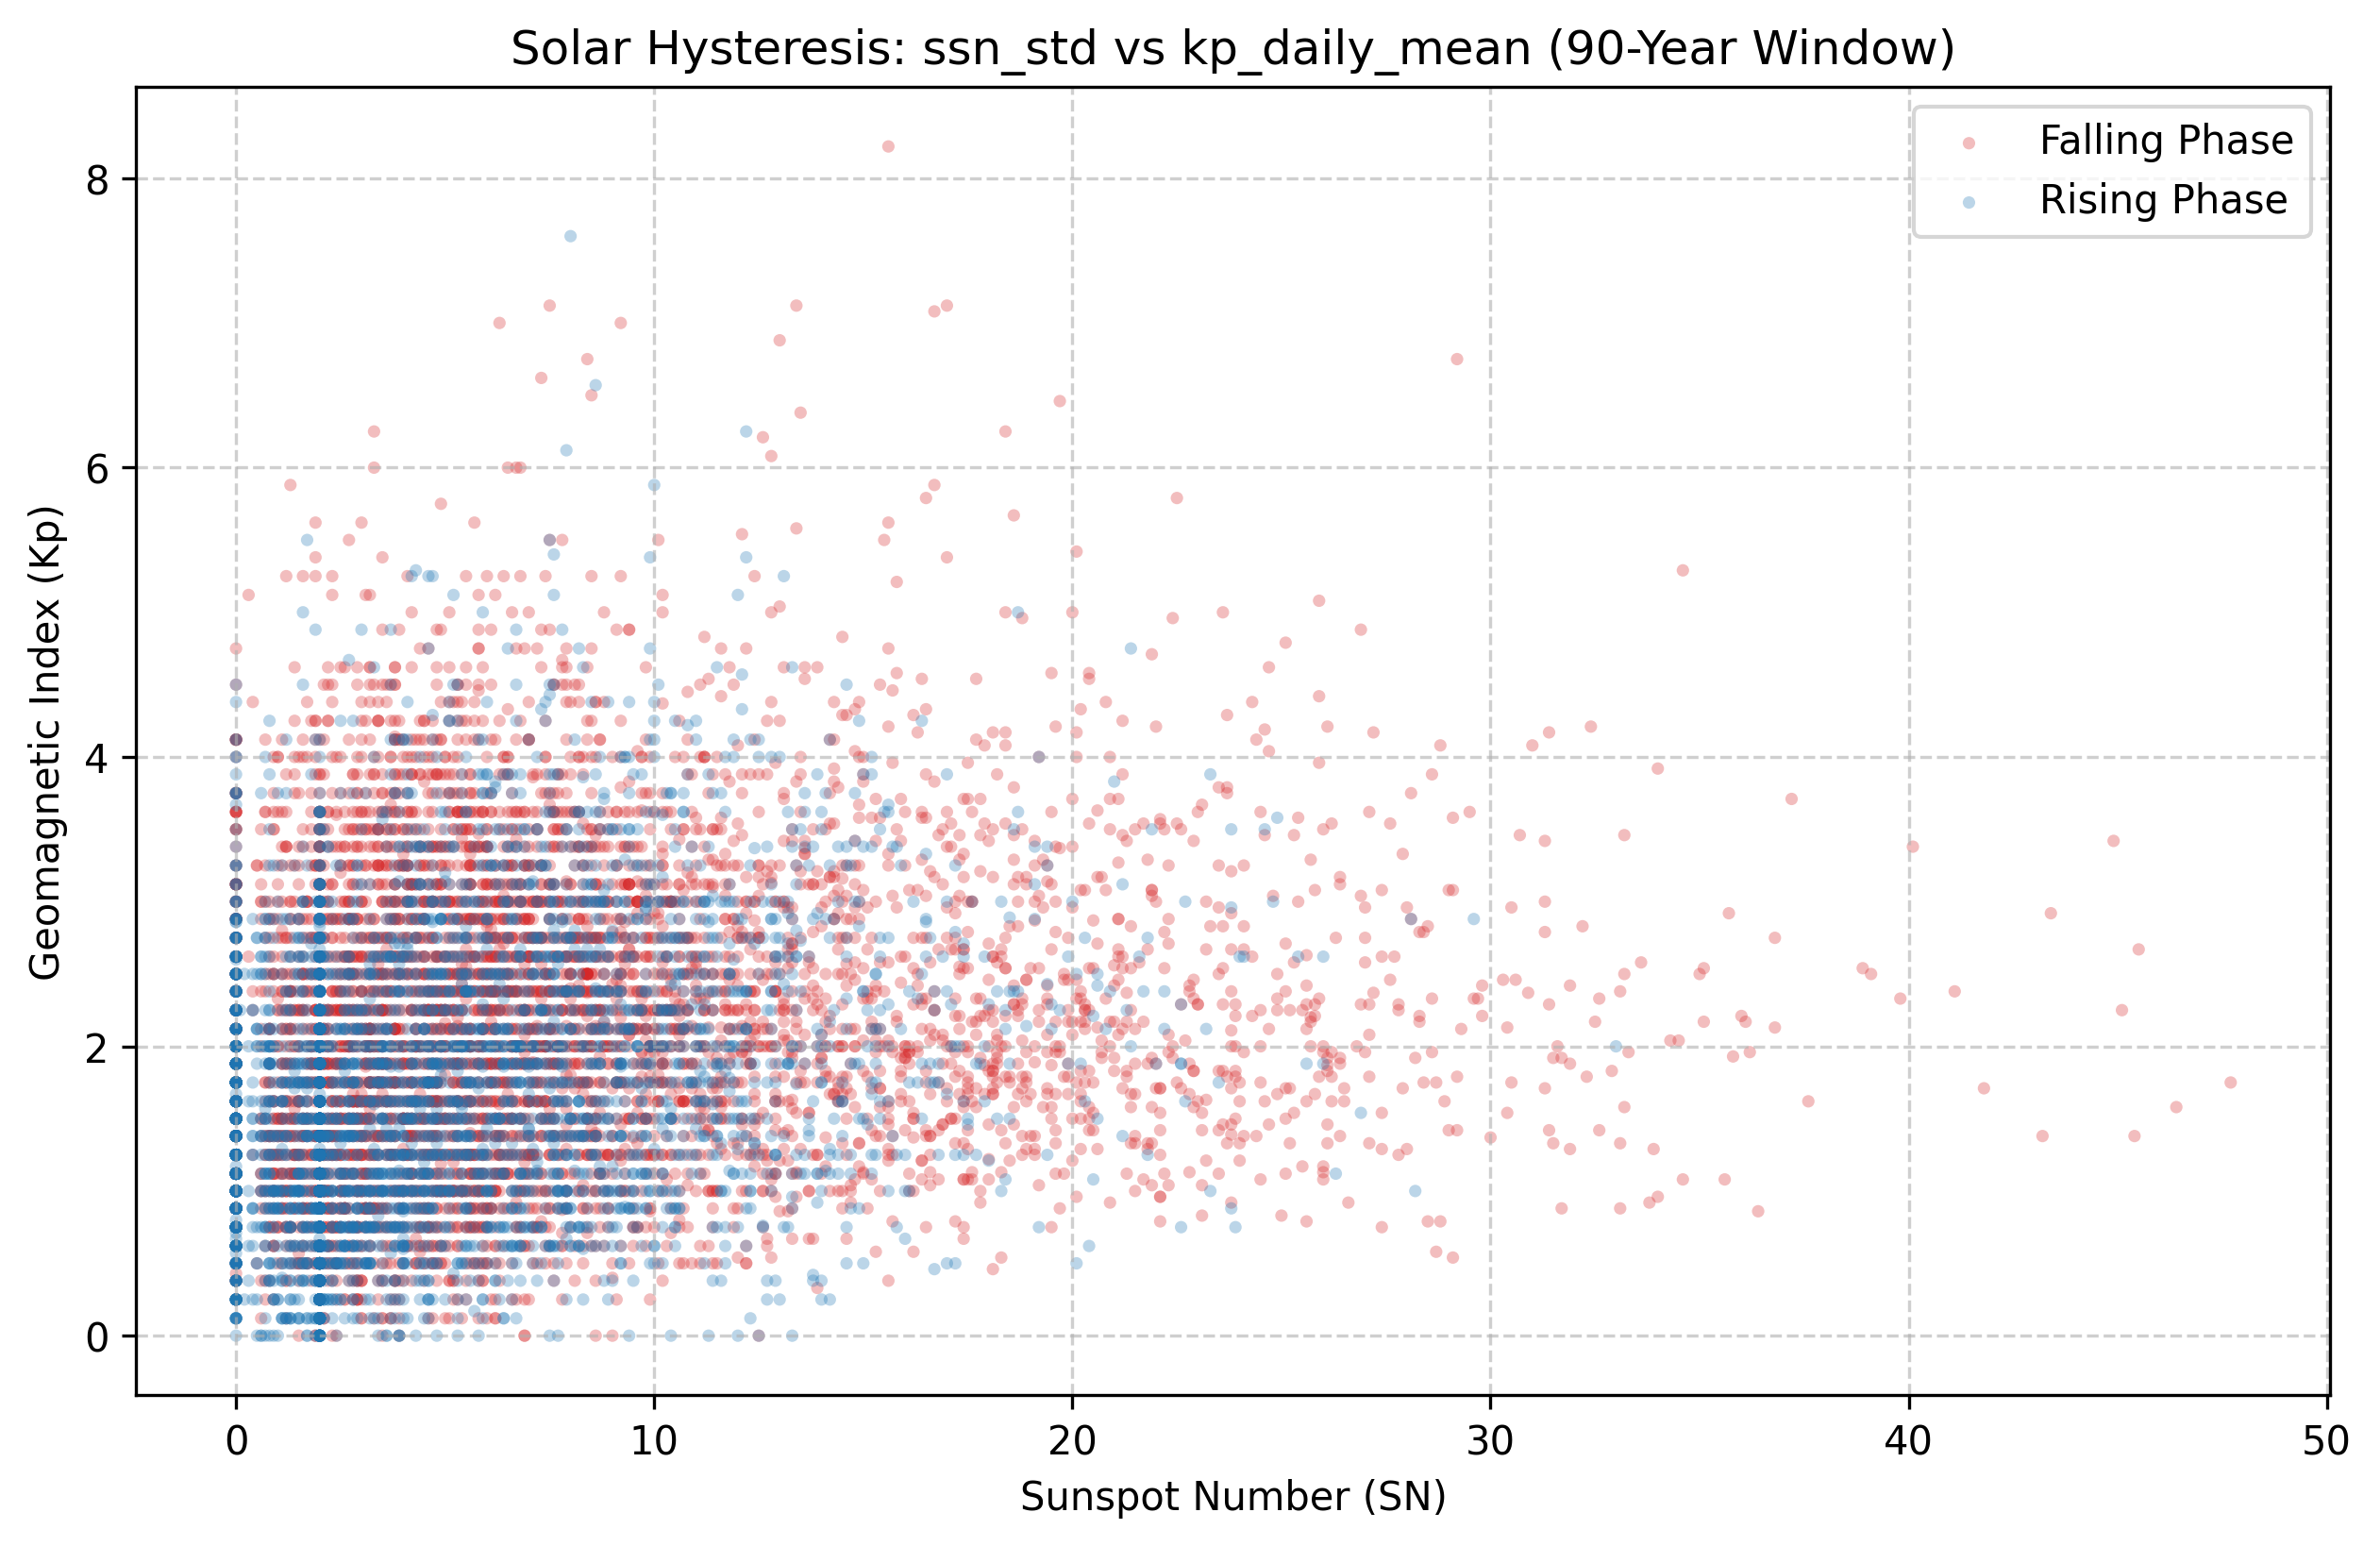
\includegraphics[width=0.85\textwidth]{./figs/hysteresis.png}
        \caption{Solar hysteresis: scatter plot of sunspot number (SSN) versus geomagnetic Kp index, colour-coded by solar cycle phase. Rising phase (blue) shows lower Kp for a given SSN compared to the falling phase (red), reflecting the delayed geomagnetic response.}
        \label{fig:hysteresis}
    \end{center}
\end{figure}

\subsection{Lead-Lag Relationships and Extreme Events}

Applying cross-correlation analysis (lag range $\pm 30$ days), we identified a characteristic lead-lag relationship where major geomagnetic responses (elevated Kp and depressed Dst) lag peaks in solar drivers (F10.7 and flares) by approximately 2 to 4 days, corresponding to the transit time of CMEs and high-speed solar wind streams. Furthermore, our anomaly detection module ($\pm 2.5\sigma$ threshold) successfully isolated historical extremes, such as the Halloween Solar Storms of October--November 2003, situating these impulsive events within the broader temporal context of Solar Cycle 23's declining phase.


\subsection{Third results: Interactive Dashboard}

The Streamlit-based analytics dashboard provides a 15-page interactive exploration environment. The home page displays five real-time KPI cards (latest SSN, F10.7 flux, Kp maximum, Dst minimum, and G1+ storm count) alongside mini time series charts with 27-day rolling averages. Users can dynamically filter the entire dataset by date range. The 15 analysis pages cover: (1) Solar Time Series, (2) System Overview, (3) Physics Primer, (4) Storm Simulator, (5) Geospatial Impact, (6) Monthly Statistics, (7) Data Smoothing, (8) Correlations, (9) Lag Analysis, (10) Periodicity, (11) Phase Climatology, (12) Hysteresis, (13) Extreme Events, (14) Data Sources, and (15) Project Details. The dashboard features a 6-hour auto-refresh mechanism and a manual ``Fetch Latest Data'' button for on-demand updates.


\section{Conclusion and Outlook}

We have presented a comprehensive Solar Activity \& Space Weather Monitoring System that addresses the fragmentation of solar/geomagnetic data by unifying five major indices from six data providers into a single, coherent analytical platform. The three-stage pipeline design ensures robustness---mirror failover and retry logic handle transient network failures, while the priority-based merging strategy and quality-controlled interpolation produce research-grade daily time series spanning nearly four decades.

Key findings from the analytical modules include the confirmation of the $\sim$11-year solar periodicity via FFT analysis, the quantification of the solar hysteresis effect showing peak geomagnetic storm probability during the declining phase of the solar cycle, and the identification of significant cross-correlation lags between solar indicators and geomagnetic response. These results demonstrate both the scientific utility and the data integrity of the platform.

Future work will focus on three directions: (i) incorporating real-time solar wind data (e.g., ACE/DSCOVR upstream measurements) to enable short-term ($<$1 hour) geomagnetic storm forecasting, (ii) implementing machine learning models (e.g., LSTM networks) for 1--3 day Kp and Dst prediction using the multi-index feature set, and (iii) expanding the dashboard with geospatial visualizations of auroral boundaries and GIC (geomagnetically induced current) risk maps for power grid operators.


\section{Acknowledgements}

We acknowledge the data providers whose open-access archives made this project possible: the SILSO team at the Royal Observatory of Belgium, NOAA's National Centers for Environmental Information (NCEI) and Space Weather Prediction Center (SWPC), GFZ German Research Centre for Geosciences (Potsdam), NASA's Space Physics Data Facility (SPDF), and the World Data Center for Geomagnetism (WDC Kyoto). We also thank the developers of the open-source Python libraries---Pandas~\citep{mckinney_pandas_2010}, Plotly, Streamlit~\citep{streamlit_2020}, NumPy, SciPy, and PyWavelets---that form the computational backbone of this system.

\textbf{Declaration of AI Usage:} In accordance with course guidelines, Large Language Models (LLMs) including Claude/Gemini were utilized as assistive tools during this project for rapid code prototyping, debugging PyWavelets integration, and refining LaTeX formatting. All AI-generated logic was rigorously validated and manually adapted to ensure correctness.


\section{Author Contributions}

\textbf{Mulumudi Dinesh Karthik} designed and constructed the Streamlit interactive dashboard, integrating real-time KPIs and 15 analytical pages. \textbf{Vansh Gupta} led the data collection efforts by identifying authoritative API endpoints and building the robust data ingestion scripts. \textbf{Abhishek Menon} developed the statistical analysis library (\texttt{analysis.py}), focusing on cross-correlation, phase-locked climatology, and periodicity detection. \textbf{Shailendra Pratap Singh} engineered the comprehensive data cleaning module, ensuring multi-source dataset harmonization, gap interpolation, and categorical storm-severity derivation. All members participated in code reviews, data validation, and collectively drafted the project report.


\section{Code availability}
The code for this project is available at the following GitHub repository:
\url{https://github.com/sharp-00/Solar-Activity-Space-Weather-Monitoring-System.git}.

% --------------------------------------------------------------------
% --------------------------------------------------------------------
% ---- DO NOT CHANGE THIS BLOCK OF CODE
\section{References}
\bibliography{refs}
% --------------------------------------------------------------------
% --------------------------------------------------------------------


\section{Appendix}

\subsection{Dashboard Screenshots}

Our completed 15-page Streamlit analytics dashboard provides extensive tools for exploring space weather phenomena. The core features highlighted include the auroral footprint mapping, real-world consequence simulation, customizable data smoothing, and global operational diagnostics.

\begin{figure}[H]
    \centering
    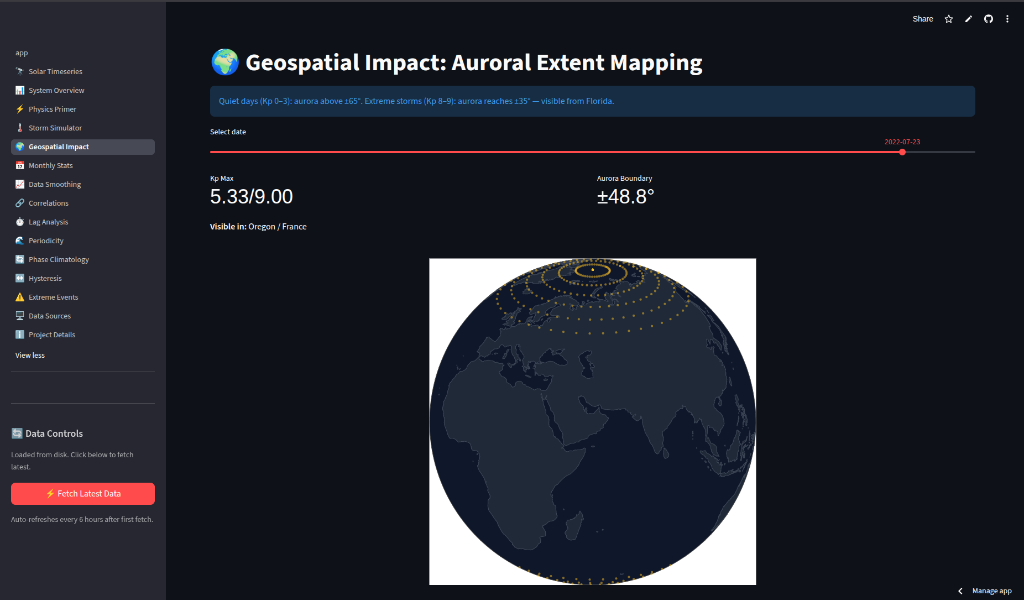
\includegraphics[width=0.9\textwidth]{./figs/dashboard_1.png}
    \caption{Geospatial Impact: The Auroral Extent Mapping page visualizes the potential geographical visibility of the aurora based on real-time and historical Kp levels.}
    \label{fig:dashboard1}
\end{figure}

\begin{figure}[H]
    \centering
    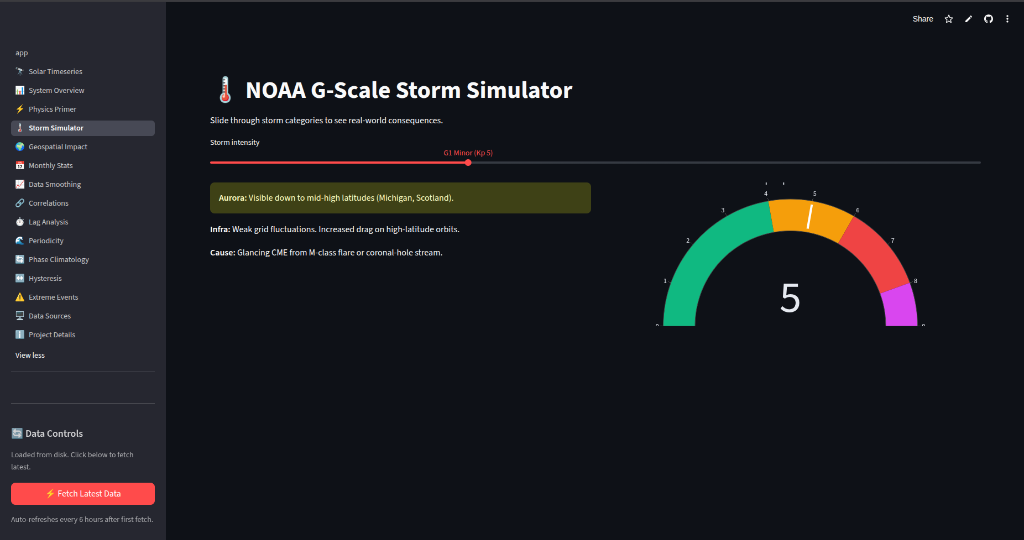
\includegraphics[width=0.9\textwidth]{./figs/dashboard_2.png}
    \caption{NOAA G-Scale Storm Simulator: An interactive educational tool allowing users to simulate various geomagnetic storm severities and observe their associated societal, infrastructural, and biological impacts.}
    \label{fig:dashboard2}
\end{figure}

\begin{figure}[H]
    \centering
    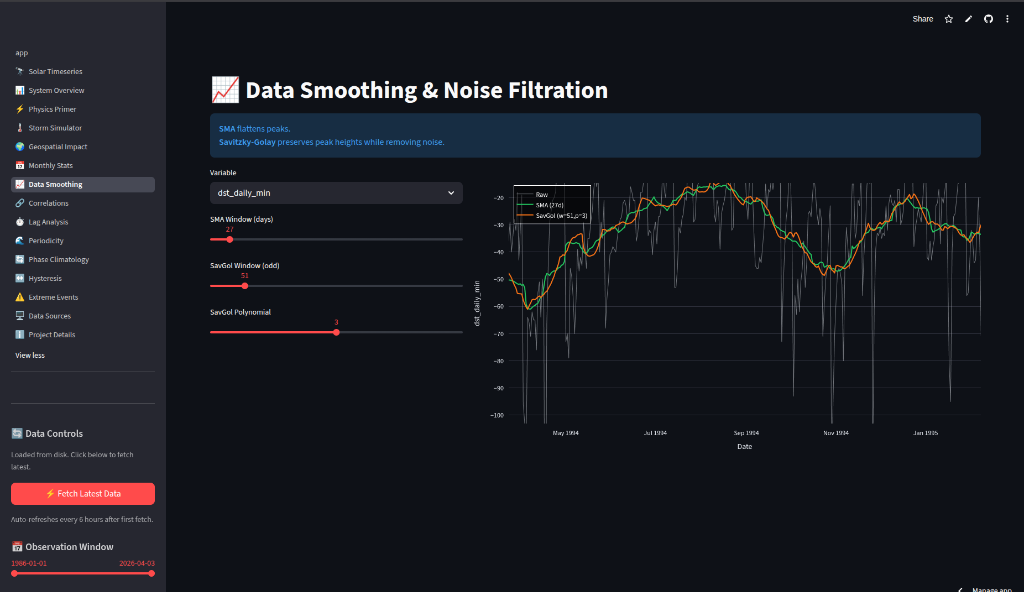
\includegraphics[width=0.9\textwidth]{./figs/dashboard_3.png}
    \caption{Data Smoothing \& Noise Filtration: Provides dynamic comparison between Simple Moving Averages (SMA) and Savitzky-Golay filtering, enabling analysts to isolate low-frequency trends from high-frequency observational noise.}
    \label{fig:dashboard3}
\end{figure}

\begin{figure}[H]
    \centering
    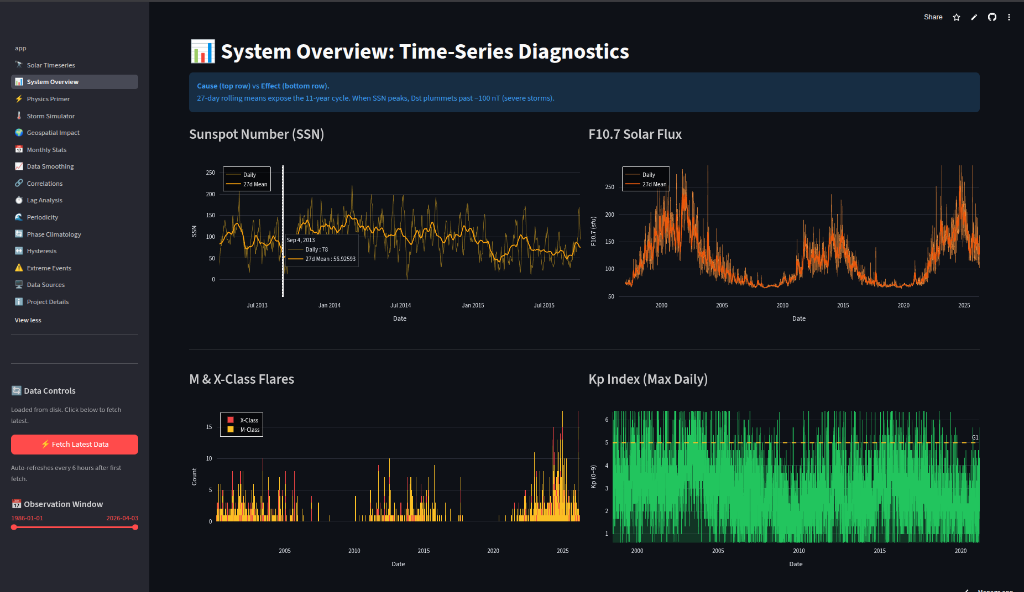
\includegraphics[width=0.9\textwidth]{./figs/dashboard_4.png}
    \caption{System Overview - Time-Series Diagnostics: The primary executive view plotting cause (SSN, Solar Flares) alongside effect (F10.7, Kp) to illustrate the solar-terrestrial energy cascade.}
    \label{fig:dashboard4}
\end{figure}

\subsection{Algorithms}

Algorithm~\ref{alg:pipeline} describes the data pipeline orchestration logic.

\begin{minipage}{0.85\textwidth}
    \begin{algorithm}[H]
        \caption{Solar Weather Data Pipeline}\label{alg:pipeline}
        \begin{algorithmic}
        \Require Raw data directory, clean output directory
        \Ensure Harmonised daily Parquet dataset
            \State \textbf{Stage 1: Ingest}
            \For{each source $s$ in $\{$SILSO, GFZ, NOAA, NASA, Kyoto$\}$}
                \For{attempt $= 1$ to $3$}
                    \State Download $s$ to \texttt{data/raw/}
                    \If{success} \textbf{break} \EndIf
                    \State Wait $5 \times \text{attempt}$ seconds
                \EndFor
            \EndFor
            \State \textbf{Stage 2: Clean}
            \For{each index $I$ in $\{$SSN, Kp, F10.7, Dst, Flares$\}$}
                \State Parse all raw sources for $I$
                \State Merge by date (newest source wins on overlap)
                \State Save $I$ as \texttt{data/clean/$I$\_daily\_clean.parquet}
            \EndFor
            \State \textbf{Stage 3: Merge}  \Comment{Build master dataset}
            \State Join all indices on date index
            \State Interpolate gaps ($\leq 7$ days linear, $\leq 3$ days forward-fill)
            \State Derive storm categories and activity labels
            \State Save \texttt{solar\_weather\_daily.parquet}
        \end{algorithmic}
    \end{algorithm}
\end{minipage}


\subsection{Code snippets}

The following snippet shows the core cross-correlation function used in our
lag analysis module:

\begin{minted}[bgcolor=white, fontsize=\small, linenos, frame=none]{python}
from scipy.stats import pearsonr

def cross_correlation(x, y, max_lag=30):
    """Pearson r between x and y at integer lags."""
    records = []
    for lag in range(-max_lag, max_lag + 1):
        if lag >= 0:
            xs = x.iloc[lag:].values
            ys = y.iloc[:len(x)-lag].values
        else:
            xs = x.iloc[:len(x)+lag].values
            ys = y.iloc[-lag:].values
        mask = ~np.isnan(xs) & ~np.isnan(ys)
        n = mask.sum()
        if n < 10:
            records.append({"lag": lag, "r": np.nan})
            continue
        r, _ = pearsonr(xs[mask], ys[mask])
        records.append({"lag": lag, "r": r, "n": n})
    return pd.DataFrame(records)
\end{minted}


% --------------------------------------------------------------------
% --------------------------------------------------------------------
% ---- DO NOT CHANGE THIS BLOCK OF CODE
\end{document}
% --------------------------------------------------------------------
% --------------------------------------------------------------------
